\chapter{Introduction}

\todo[inline]{Add references}
\todo[inline]{Change `device/computer activity' -> `task'?}
\todo[inline]{Change `natural(istic)' -> `organic'?}

% How to write an introduction: https://student.unsw.edu.au/introductions

% Move 1 establish your territory (say what the topic is about)

The rise of computing over the last half century has led to an unprecedented rise in new methods for data acquisition and analysis. However, our ability to quantify and analyse brain function is still limited. With advanced and expensive equipment, such as \emph{magnetic resonance imaging} (MRI) scanners and high-density \emph{electroencephalography} (EEG) headsets, we can record brain activity at an adequate resolution to draw conclusions about neural activation patterns under different behaviours.

While this professional-grade equipment is still unavailable to the general public, in recent years some brain imaging techniques have become commercialized for various purposes (such as meditation aids, biofeedback) and sold as consumer devices. Consequently, the cost of EEG devices has fallen sharply, offering a feasible solution to monitor brain activity in a wide range of situations to answer a range on scientific questions relating to brain activity during different tasks.

% Move 2 establish a niche (show why there needs to be further research on your topic)
% Niche 1: using automated time tracking
% Niche 2: code vs prose comprehension

Here we introduce an automated time tracker, tracking the computer activities a subject engages in, to study brain activity during a wide variety of computer-based tasks.

Studying brain activity during computer-based tasks is of particular interest to software engineers. For example, research has been done on:

\begin{itemize}
    \item Studying differences in code- and prose-comprehension~\cite{floyd_decoding_2017}\cite{fucci_replication_2019}.
    \item Measuring the difficulty of a development task~\cite{fritz_using_2014}.
    \item Minimizing interruptions~\cite{zuger_reducing_2017}.
    \item Recognizing emotions during programming~\cite{girardi_recognizing_2020}.
\end{itemize}

% other formulation of goals: profits, productivity, sustainability

% In the field of software engineering research

% This becomes especially relevant for knowledge workers, in particular software developers, who spend the vast majority of their time working on computers.

% Brain imaging techniques such as EEG show a potential to shed light on many of these research questions, and the relationship between device usage and brain activity seems an largely unexplored area worth investigating.

\todo[inline]{Move this paragraph elsewhere}

Some communities, like the Quantified Self movement, have risen to the challenge of collecting and analyzing personal data for insights into our lives and health. But while some data is easily observed (such as device usage, location, and physical movement), it remains difficult to collect data about subjective attributes (like mood, focus). To collect data on these more elusive phenomena, researchers and individuals have to resort to manual data collection like questionnaires, or approximations constructed from other data, leading to significant time costs and scaling difficulties.\cite{malhi_promise_2017}

% The purpose of this study is to investigate the feasibility of using low-cost biosensors...

% TODO: Mention brain computer interfaces at least once

% Technologies such as EEG have shown promise as early \emph{brain computer interfaces} (BCIs). The body of BCI research centers around using EEG as an input device, while \todo{really?}{less attention} has been paid to understanding how the brain behaves during various computer activities.

% Move 3 introduce the current research (make hypotheses; state the research questions)

% The contributions of this study are...

To summarize, we have in this thesis developed a framework and tooling for studying brain activity during uncontrolled device use (\emph{naturalistic device activities}). We do so by collecting brain activity data using consumer-grade EEG devices while simultaneously tracking the device activity they're engaging in. We then use the data to train machine learning models to predict the task engaged in based on the EEG readings of brain activity.

We also apply similar methodology to a controlled experiment where we present a small number of subjects with a set of code- and prose-comprehension tasks while being monitored with EEG\@. We use the collected data to train a classifier, evaluating the feasibility of EEG to distinguish between the two tasks, and use the results as an indication whether it could extend to other tasks.

% Brain Computer Interfaces (BCIs) have become available as consumer goods, thanks to the economic viability of brain imaging techniques like electroencephalography (EEG). These devices promise to measure different aspects of your mental state: wether you're grasping an object, or how calm you are during your meditation session. Low-cost brain imaging technologies like EEG are therefore suitable as candidates for richer collection about the user's mental state.

%\add[inline]{Add connection to software developers}

\section{Functional brain imaging}

    Functional brain imaging methods such as fMRI\footnote{Functional Magnetic Resonance Imaging}, fNIRS\footnote{Functional Near-InfraRed Spectroscopy}, and EEG, have been used to study the relationship between cognitive or physical activity, and brain activity~\cite{floyd_decoding_2017}\cite{hong_classification_2015}\cite{fucci_replication_2019}. 

    The more accurate methods, such as fMRI, are costly and inflexible/impractical for many uses. The different methods in general come with an array of trade-offs. The most common one is cost: operating an fMRI machine costs on the order of \$300/h~\cite{fucci_replication_2019}. 

    Other considerations when picking a brain imaging method is temporal/spatial resolution. For instance, fMRI can measure activity deep in the brain (good spatial resolution), but has difficulty tracking activity over time due to relying on blood oxygenation, which is a much slower process than the underlying neural processes (bad temporal resolution)~\cite{glover_overview_2011}. EEG on the other hand, has excellent temporal resolution (usually sampled at about 256Hz), but it can't reliably discern activity deep in the brain (bad spatial resolution, partially depending on channel count), but.

    Recently, the availability and cost reduction of biosensors such as EEG, HEG\footnote{Hemoencephalography}, and fNIRS, has enabled studying brain activity during real-life tasks. This is the opportunity we seek to take advantage of, and as EEG is the most well developed of the three, we choose it for our investigation.

    EEG works by measuring tiny amounts of electricity (on the order of microvolts) on the scalp to listen to the underlying firing of neurons. By placing electrodes in various configurations, information about the activity of different brain regions can be inferred. The extent of how much information can actually be decoded from the signal remains an open research question.

    But EEG is not without its limitations --- among them a notably low signal-to-noise ratio~\cite{mcfarland_eeg-based_2017}, as well as being difficult to use for discerning activity deeper in the brain~\cite{fahimi_hnazaee_localization_2020} --- yet these limitations have been overcome for many applications, like ERP experiments, and has even turned out prove sufficient for high-speed BCI applications through detecting visual evoked potentials (VEPs)~\cite{spuler_high-speed_2017}.

    To combat the low signal-to-noise ratio, machine learning methods have been employed with varying degrees of success. Examples from previous research include Convolutional Neural Networks (CNNs), which have been successful in classifying time series in general~\cite{zhao_convolutional_2017}, and EEG data in particular~\cite{schirrmeister_deep_2017}. As well as Hierarchical Convolutional Neural Networks (HCNNs), which have been used for EEG-based emotion recognition~\cite{li_hierarchical_2018}.

    \subsection*{Cost reduction}

    The cost-reduction of EEG devices took hold in 2013, when OpenBCI ran the founding crowdfunding round on Kickstarter. During the campaign, they offered their 16-channel Cyton + Daisy board (seen in figure~\ref{fig:cyton}) for \$549\footnote{Fun fact: I funded them at one of the lower tiers back then.}~\cite{noauthor_openbci_nodate}.

    The commercialization of EEG towards a general audience was furthered by InteraXon with the release of the original Muse in 2016. Aimed at meditation practice, it was the first consumer-oriented EEG device on the market. Later, in 2019, InteraXon released the Muse~S (as seen in~\ref{fig:museS}), a headband-style EEG headset developed for sleep and longer sessions.

    In 2020 and 2021, the company Neurosity has released their 8 channel Crown headset (seen in figure~\ref{fig:crown}), targeted at developers and knowledge workers to `shift into focus'.

    More recently, projects like the FreeEEG32 offer a 32 channel board for only \$199, expected to ship in 2022.\cite{noauthor_freeeeg32_nodate}

    \subsection*{Applications in neurolinguistics}

        EEG has found many applications in neurolinguistics, both to understand how the brain processes natural languages as well as programming languages~\cite{prat_relating_2020}.

         As an example it has been shown that it is possible to classify if a participant is reading code or prose using fMRI~\cite{floyd_decoding_2017}, which has been replicated using EEG and low-cost biosensors~\cite{fucci_replication_2019}. The ability to distinguish between these two tasks have been has been explained neurologically by the recruitment of different neural networks in the brain~\cite{ivanova_comprehension_2020}.

        The code vs prose comprehension task has also been modified into a writing task studied under fMRI, to further shed light to the underlying brain activity. In one study it was found that code and prose writing are significantly dissimilar tasks for the brain, where prose writing engages brain regions associated with language in the left hemisphere while while code writing engages brain regions associated with attention, working memory, planning, and spatial cognition in the right hemisphere\cite{noauthor_neurological_nodate}. To study this with MRI, the authors had to use (develop?) an MRI-safe keyboard.

        As far as I know, code vs prose \emph{writing} has not been studied with EEG\. However, using ActivityWatch and other tools we've developed in this thesis (like the input watcher) one can to distinguish whether the user is reading or writing, as well as whether they're working with code or prose, which enables studying the same activities in a naturalistic setting.

    % Moved earlier in the introduction
    %\subsection*{Applications in software engineering}

    % https://docs.openbci.com/citations

    % List of functional brain imaging techniques:
    %  - fMRI
    %  - fNIRS
    %  - EEG
    %  - HEG


\section{Automated time trackers}

    People spend more time than ever using computing devices. Work, entertainment, and services, have been steadily moving online over the last few decades and this trend is expected to continue.
    While several studies have been tracking how people spend time on their devices, a wider study of how people's app usage is changing over time, and how it varies with demographics, is not publicly available.

    Furthermore, how different device activities affect the user behaviorally and neurologically is of interest for many areas of research, including:

    \begin{itemize}
        \item psychological well-being, such as depression and social anxiety~\cite{selfhout_different_2009}\cite{shah_nonrecursive_2002}, stress~\cite{mark_stress_2014}, self-esteem, life satisfaction, loneliness, and depression~\cite{huang_time_2017}.
        \item the impact of screen time on children and adolescents~\cite{subrahmanyam_impact_2001}.
        \item attention span among media multitasking adults~\cite{mark_stress_2014}.
        \item enhancing personal productivity~\cite{kim_timeaware_2016}.
    \end{itemize}

    Understanding device use and the underlying cognitive processes are essential when designing for motivation, engagement and wellbeing in digital experiences~\cite{peters_designing_2018}.

    Automated time-trackers have been developed for computing devices, with various applications such as tracking hours worked, personal productivity, managing excessive use of social networking sites (SNSs), and studying human behavior.

    This section introduces how such devices are used in commercial services and in research. Finally, we present the open source solution ActivityWatch.

    \subsubsection*{Commercial use}

        Companies like RescueTime~\cite{noauthor_rescuetime_nodate}, Hubstaff~\cite{noauthor_hubstaff_nodate}, and others offer automated time tracking as a service. These services track users' screen time using an application which tracks the active application, and sends the data to their servers for storage and analysis. The user can then view their data in a dashboard on the services' website. Many of these services are marketed towards professionals who want to keep track of individual and team productivity.

        However, these services have some issues for use by researchers and individuals alike. Notably, their collection of detailed and non-anonymized behavioral data into a centralized system bring significant privacy concerns, especially in cases where the data is shared with a team or an employer.

        Other limitations of these services, such as low temporal resolution and limited event detail, cause additional issues for certain tasks that are timing-sensitive (such as ERPs), or preprocessing steps that can take advantage of high level of detail (like classifying activity).

    \subsubsection*{Research use}

        Previous research has been published which used automated time trackers, such as TimeAware~\cite{kim_timeaware_2016} and ScreenLife~\cite{rooksby_personal_2016}. However, these previous contributions are --- like the commercial services --- not open source nor permissively licensed, and therefore not available for external research use nor further development.

    \subsubsection*{ActivityWatch}

        The free and open source automated time tracker ActivityWatch~\cite{bjareholt_activitywatch_2020}, previously developed by the author of this thesis together with contributors, addresses aforementioned issues with other software around source availability/licensing, privacy, temporal resolution, event detail, and cross-platform support.

        \todo[inline]{Update screenshot to v0.11}

        \begin{figure}[h]
        \centering
        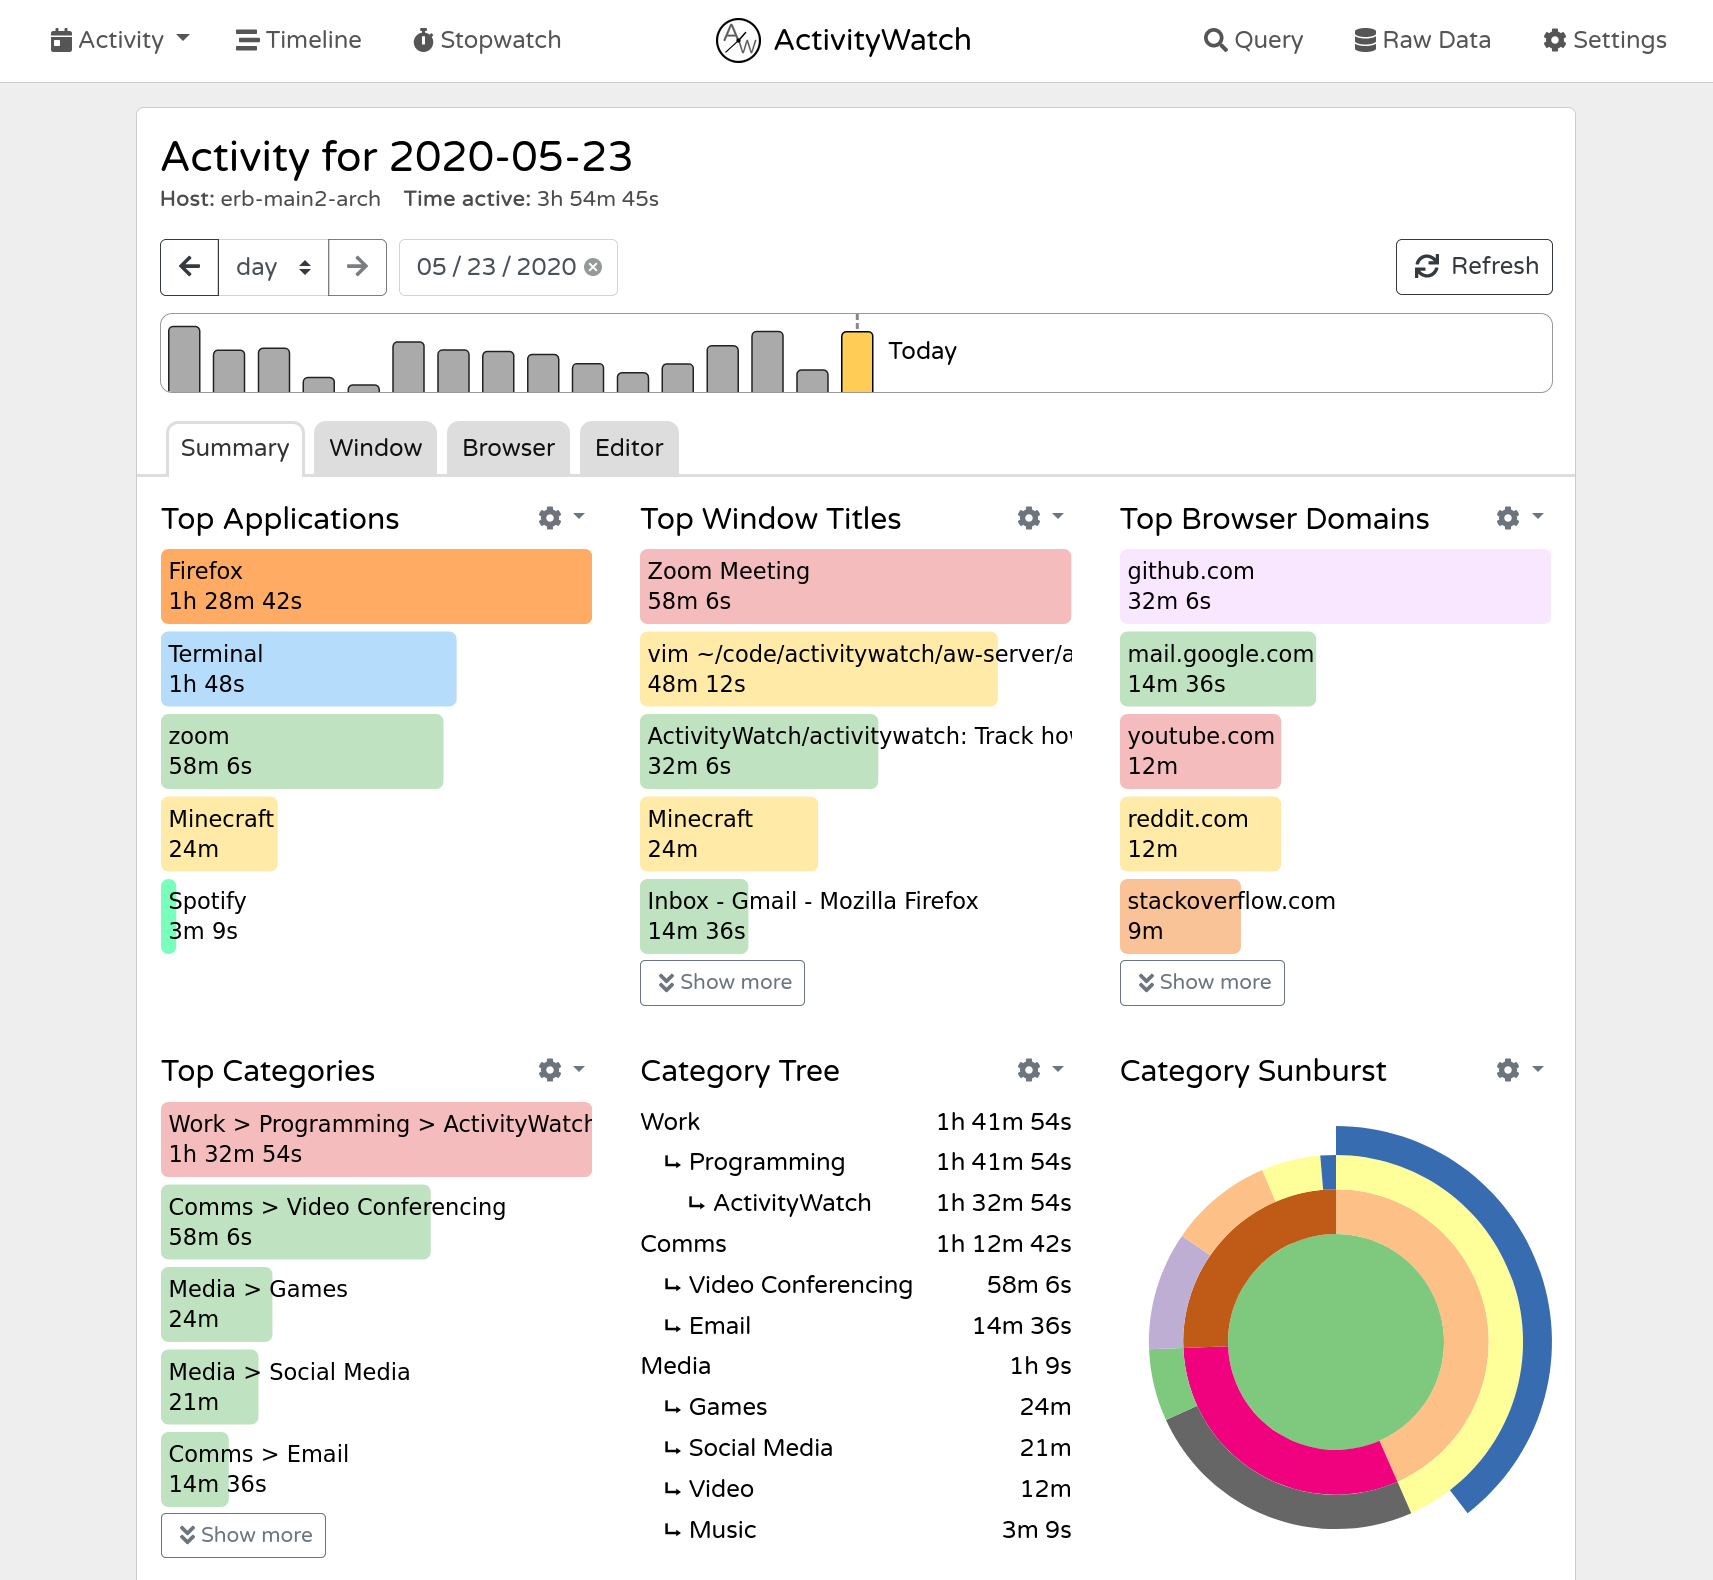
\includegraphics[width=12cm]{img/screenshot-aw-activity.png}
        \caption{ActivityWatch activity dashboard. Showing top applications, window titles, browser domains, and categories.}\label{fig:aw}
        \end{figure}

        ActivityWatch as a project was started in 2016 by the author of this thesis, with his brother Johan joining development soon after. It has since become a popular open source alternative to other time tracking software. It has received numerous contributions from users\footnote{Contributor statistics available at \href{https://activitywatch.net/contributors/}{activitywatch.net/contributors/}} and is approaching 100,000 downloads\footnote{Download statistics available at \href{https://activitywatch.net/stats/}{activitywatch.net/stats/}}.

        \todo[inline]{What more could I add about ActivityWatch? There should be relevant stuff in the docs, and in the slides I made way back.}

\section{Aim of the thesis}

    \todo[inline]{Make align with goaldoc}

    The primary aim of the thesis is to improve upon previous attempts~\cite{fucci_replication_2019} to classify whether the user is reading code or prose using EEG data. This is to be achieved by using better EEG equipment and explore state of the art analysis methods, such as Riemannian geometry and neural networks.

    The secondary aim of the thesis is to investigate whether the ability of EEG analysis to classify code vs prose comprehension generalizes across more activities, such as the wide variety of tasks engaged in during natural device use.

    Additional aims of the thesis include:

    \begin{itemize}
        \item Develop a method for automatically labelling EEG data using ActivityWatch
        \item Providing a complete reproduction package, including all code and data.
        \item Improving open-source tools for EEG analysis.
    \end{itemize}

    \add[inline]{Insert stuff from goal document}

\section{Related work}

    Farias et al.\ conducted a systematic mapping study which reviews the usage of psychophysiological data in software engineering~\cite{vieira_usage_2021}.

    Previous research shows that fMRI (by Floyd et al.~\cite{floyd_decoding_2017}) and EEG (by Fucci et al.~\cite{fucci_replication_2019}) can be used to classify whether a subject is reading prose or code. However, accuracy with single-channel EEG has been found to be poor, and notably outperformed by a heart rate variability (HRV) monitor.

    % Here, we used functional magnetic resonance imaging to investigate two candidate brain systems: the multiple demand (MD) system, typically recruited during math, logic, problem solving, and executive tasks, and the language system, typically recruited during linguistic processing.
    Recently, it has been shown that the multiple demand (MD) system\footnote{A set of frontoparietal brain regions involved in diverse tasks} is typically recruited for code comprehension tasks, as opposed to the language system\footnote{Specialized brain regions that respond selectively during language processing} that is typically recruited during prose comprehension~\cite{ivanova_comprehension_2020}. This sheds light on the significant differences in how the brain processes code vs prose.

    In addition to purely studying comprehension (reading) code and prose, an 2020 fMRI study showed that there are indeed significant neurological differences between \emph{writing} code and prose as well~\cite{noauthor_neurological_nodate}.

    In software engineering research, low-cost biosensors such as wristbands that measure electrodermal activity and heart-related metrics have been used for emotion detection, as a tool in studying developer productivity~\cite{girardi_recognizing_2020}.

    %\add[inline]{Insert mention of preprint that Fucci mentioned?}
